\chapter{Risoluzione del problema tramite CPLEX}\label{CPLEX}  

\section{Modelli compatti}
I modelli compatti del Travelling Salesman Problem, sono formulazioni il cui numero di variabili e di vincoli è polinomiale nella taglia dell'istanza. In particolare, in quelle analizzate in seguito, sono entrambi $O(n^2)$, con \textit{n = numero di nodi}.\\
I modelli compatti sono però applicabili solo a grafi orientati. Per poterli sfruttare per la risoluzione del TSP simmetrico, è necessario per ogni ramo dell'istanza $(i,j)$, inserire nel modello i corrispondenti rami orientati in entrambe le direzioni $(i,j)$ e $(j,i)$. Questo comporta un significativo rallentamento nella computazione della soluzione, in quanto l'algoritmo, ogni volta che scarta un ramo $(i,j)$ dalla soluzione ottima, verifica se il corrispondente $(j,i)$ potrebbe invece appartenerle. Questo non può però essere possibile, essendo i due rami in realtà lo stesso nella nostra istanza iniziale.
\subsection{Formulazione sequenziale}
Miller, Tucker e Zemlin, nella loro formulazione del modello, hanno introdotto una nuova variabile $u_i$ per ogni nodo \textit{i} e imposto che, nella soluzione ottima, il suo valore  rispettasse dei nuovi vincoli. Questi servivano a garantire che venisse seguito un ordine di percorrenza di tutti i nodi. In questo modo hanno eliminato la creazione di sub-tour, mantenendo il numero di vincoli e di variabili polinomiale. Nello specifico il loro modello è così strutturato:
\begin{align}
& min \underset{i\in V}\sum{}\underset{j\in V}\sum{c_{i,j}\; x_{i,j}} \\ \notag \\
& \underset{i\in V}\sum{x_{ih}}\; =\; 1 & \forall\; h\in V \\ \notag \\
& \underset{j\in V}\sum{x_{hj}}\; =\; 1 & \forall\; h\in V \\ \notag \\
& u_i-u_j+n\; x_{i,j}\;\leq\; n-1 & \forall\; i,j\in V-\{ 1\} , i\neq j \\ \notag \\
& 0\leq u_i\;\leq\; n-2 & \forall\; i\in V-\{ 1\} \\ \notag 
\end{align}
Esistono due diversi modi per implementare questo modello sfruttando le funzioni di CPLEX.\\
Nel primo i nuovi vincoli vengono aggiunti come visto in precedenza. In questo modo, durante la fase di preprocessamento, il programma è già a conoscenza di tutti i vincoli che dovrà rispettare la soluzione ottima. Ciò gli permette di migliorare i coefficienti presenti, prima ancora di iniziare la computazione dell'ottimo.\\
Il secondo metodo, invece, sfrutta l'inserimento nel modello di vincoli detti "lazy constraints". Questi non sono noti al programma dall'inizio, ma vengono inseriti all'interno di un pool di vincoli. Nel momento in cui viene calcolata una soluzione, CPLEX verifica che vengano rispettati tutti i vincoli presenti nel pool. Se ne trova uno violato lo aggiunge al modello e ripete la computazione. Questo approccio permette, per risolvere lo stesso problema, di eseguire calcoli su un modello più piccolo, ma può aumentare i tempi di computazione non fornendo a CPLEX tutte le informazioni dall'inizio.   

\subsection{Formulazione basata sul flusso}
Nella formulazione di Gavish e Graves, per impedire la formazione di sub-tour all'interno della soluzione ottima, viene introdotto un nuovo vincolo per ogni ramo del grafo. Questo permette di regolare il flusso $y_{i,j}$, con $i\neq j$,  che lo attraversa.Inoltre è stato necessario aggiungere anche dei vincoli, detti "vincoli di accoppiamento", che collegassero i flussi alle variabili $x_{i,j}$ . Il loro modello è quindi così strutturato:
\begin{align}
& min\underset{i\in V}\sum{\underset{j\in V}\sum{c_{i,j}\; x_{i,j}}} \\ \notag \\
& \underset{i\in V}\sum{x_{ih}}\;=\;1 & \forall\;h\in V \\ \notag\\
& \underset{j\in V}\sum{x_{hj}}\;=\;1 & \forall\;h\in V \\ \notag\\
& \underset{j\in V}\sum{y_{1,j}}\;=\;1\\ \notag\\
& \underset{j\in V}\sum{y_{h,j}}\;=\;\underset{i\in V}\sum{y_{i,h}}\;-1 & \forall\;h\in V-\{1\}\\ \notag\\
& y_{i,j}\leq\;(n-1)\;x_{i,j} & \forall\;i,j\in V, i\neq j\\ \notag
\end{align}
La soluzione di questo modello risulta però essere lontana dalla convex hull. Per migliorarla è possibile sostituire il vincolo \textit{(3.11)} con \\
\begin{center}
$y_{i,j}\leq\;(n-2)\;x_{i,j} \;\;\;\;\;\forall\; i\neq \; j$\\
\end{center}
mentre per gli altri valori di $i$ e $j$ è necessario lasciare i vincoli originali. 
Per evitare che la soluzione ottima contenga sia l'arco $x_{i,j}$ che $x_{j,i}$, che nella nostra istanza iniziale corrispondono allo stesso arco, viene anche aggiunto il seguente vincolo:
\begin{center}
$x_{i,j}+x_{j,i}\leq 1\;\;\;\; \forall i,j \in V$ con $i < j$
\end{center}

\section{Loop}
\subsection{Formulazione di Benders}
Negli anni '60, Jacques F. Benders sviluppò un approccio generale, applicabile a qualsiasi problema di programmazione lineare, per ridurre il numero esponenziale di alcuni vincoli specifici inseriti nel modello.\\
Utilizzando questo metodo, il modello viene scritto senza quei vincoli e poi questi verranno aggiunti in seguito durante la risoluzione del problema. Nel caso in cui la soluzione ottima, calcolata a partire da questo modello, non rispetti un vincolo di quelli rimossi, questo viene aggiunto al modello. \\
Nella seguente parte, viene riportata l'applicazione specifica di loop al problema TSP.
I vincoli di Subtour Elimination sono in numero esponenziale e sono:\\
\begin{align}
&\underset{e\in E(S)}\sum{x_{e}} \leq \mid S\mid - 1\;\forall\;S\underset{\neq}{\subset}V\; : \; \mid S\mid\geq 2
\end{align}
o equivalentemente:
\begin{align}
&\underset{e\in \delta(S)}\sum{x_{e}}\geq 2\;\forall\;S\underset{\neq}{\subset}V\; : \; \mid S\mid\geq 2
\end{align}
Viene definito un nuovo modello per il problema del commesso viaggiatore simmetrico, in cui vengono rimossi tali vincoli, aggiungendo così la possibilità di avere dei subtour nella soluzione finale.\\
Viene risolto il problema e nel caso in cui ci sia più di una componente connessa, viene aggiunto al modello un vincolo di subtour elimination per ogni 
ciclo generato.\\
\begin{algorithm}[H]
\DontPrintSemicolon
\KwIn {$\mathtt{model}$= Modello TSP simmetrico senza vincoli di Subtour Elimination\newline}
\KwOut {$\mathtt{x}$= soluzione intera senza subtour}
\BlankLine 
 $\mathtt{x} \gets$ solve(model)\;
 $\mathtt{ncomps} \gets$ comps(x)\;
 \BlankLine 
 \While{$\mathtt{ncomps} \geq 2$}{
  Aggiungi $\underset{e\in \delta(S_k)}\sum{x_{e}}\leq \mid S_k\mid - 1\;\forall$ componente connessa $S_k$\;
  \BlankLine  
  \If{$\mathtt{ncomps} \geq 2$}{
    \BlankLine
    $\mathtt{x} \gets$ solve(model)\;
    $\mathtt{ncomps} \gets$ comps(x)\;
  }
 }
 \caption{LOOP}
\end{algorithm}

All'aumentare del numero di vincoli, il costo della soluzione ottenuta da CPLEX peggiora o resta identica a quella elaborata all'iterazione precedente del metodo loop.\\
Il numero di iterazioni che vengono effettuate dall'algoritmo non è conosciuto e potrebbe essere anche molto elevato. Nel caso peggiore vengono inseriti tutti i vincoli di Subtour elimination, ovvero un numero esponenziale di disequazioni, soprattutto con istanze clusterizzate.\\
Inoltre il problema principale di questo algoritmo è la generazione, ad ogni iterazione, di un albero completo di branching, eliminando quello precedentemente sviluppato.\\
In passato, con le versioni del MIP solver di CPLEX degli anni '60, questa operazione era molto onerosa mentre attualmente il metodo loop garantisce la risoluzione, anche di istanze molto grandi, in tempi ragionevoli.
Questo non accade invece per il Branch \& Bound in quanto vengono aggiunte nuove ramificazioni all'albero già esistente.\\
L'introduzione di nuovi vincoli di Subtour Elimination, solo nel momento in cui si presenta una loro violazione, permette di ridurre la dimensione del modello ma riduce l'attività di pre-processamento svolta da CPLEX prima di cominciare la risoluzione del problema. Nella fase di pre-processing infatti, vengono applicati algoritmi euristici e cambiamenti dei coefficienti nel modello, in base ai vincoli inseriti.\\
L'algoritmo può essere modificato svolgendo prima il metodo loop con l'aggiunta di parametri differenti da quelli utilizzati di default del risolutore CPLEX. In seguito viene effettuato nuovamente l'algoritmo di Benders ma questa volta nella sua versione esatta, in modo da migliorare la soluzione meta-euristica trovata nella prima parte. \\
Quest'ottimizzazione è basata sul fatto che CPLEX salvi alcune soluzioni, ottenute in precedenza dal risolutore sullo stesso modello, e le sfrutti come bound nel nuovo modello. Per questo motivo, alcune delle soluzioni metaeuristiche ottenute nella prima fase vengono sfruttate come bound nella seconda.

\subsection{Formulazione con callback}
Un possibile miglioramento dell'algoritmo proposto da Benders, in termini di velocità della computazione, è il seguente.\\
Come precedentemente descritto, come prima cosa CPLEX effettua un preprocessamento in cui semplifica il modello, riducendo il termine noto e accorpando tra loro diverse variabili. Terminata questa operazione inizia ad eseguire la fase di Branch \& Cut. Ogni volta che calcola una nuova soluzione $x^*$, prima di dichiarare se è l'ottimo o di scartarla e proseguire a sviluppare i successivi rami dell'albero decisionale, applica dei tagli e degli algoritmi euristici per aggiornarla(vedi Figura \ref{Albero_decisionale}).
\begin{figure}[h] 
\begin{center} 
  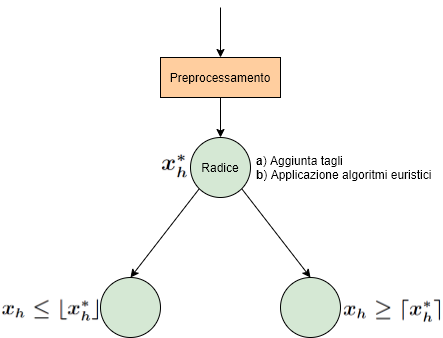
\includegraphics[scale=0.7]{Images/albero_decisionale}\\ 
  \caption{\footnotesize{Albero decisionale del Branch and Cut}}
  \label{Albero_decisionale} 
\end{center} 
\end{figure}
\\Nello sviluppo di ogni ramo l'upper bound sarà dato dagli algoritmi euristici utilizzati, mentre il lower bound dal rilassamento del problema.\\ 
Per poter velocizzare l'approccio proposto da Benders, è possibile personalizzare questa fase e scegliere quali tagli far applicare a CPLEX. Nel nostro caso, questi vengono utilizzati per eliminare l'eventuale presenza di subtour nella soluzione calcolata. Per fare ciò vengono sfruttate particolari funzioni fornite da CPLEX, dette \textit{callback}. Queste sono state lasciate volutamente vuote dai creatori della libreria, affinché l'utente possa implementarne all'interno il suo specifico codice. In particolare, le funzioni utilizzate sono callback necessarie ad aggiungere lazy constraints al modello e per questo dette \textit{lazy constraints callback}. La callback implementata viene chiamata solo al momento di aggiornare l'incumbent e se necessario aggiunge al modello i vincoli violati. Verrà quindi invocata più frequentemente all'inizio del calcolo della soluzione del problema, e meno nelle iterazioni successive. Questo poichè essendoci in partenza meno vincoli, sarà più facile per la soluzione soddisfarli tutti. A differenza dei \textit{lazy constraints}, con l'utilizzo delle \textit{lazy callback} i vincoli non sono costantemente presenti in un pool, ma vengono generati "al volo" al momento necessario.  Quest'operazione velocizza notevolmente il calcolo della soluzione ottima, in quanto permette a CPLEX di non dover calcolare nuovamente l'albero decisionale dalla radice, ma di proseguirne lo sviluppo aggiungendo nuovi rami. In particolari casi, però, CPLEX può ritenere più conveniente distruggere tutto l'albero decisionale fin'ora calcolato e ricominciare dalla radice. Questo può avvenire in qualunque punto dell'elaborazione della soluzione ottima.\\
Attraverso l'utilizzo delle callbacks è possibile accedere a molti dati interni all'elaborazione di CPLEX. Particolari procedure vengono quindi automaticamente disattivate, affinché l'utente non possa venirne a conoscenza. Per evitare questo è possibile installare le callbacks con una modalità leggermente diversa, attraverso funzioni dette \textit{general}.
\section{Algoritmi Math-Heuristic}
Gli algoritmi euristici sono progettati per risolvere istanze del problema in tempi significativamente più brevi rispetto agli algoritmi esatti. Di conseguenza, però, al termine della computazione non garantiscono di ottenere una soluzione ottima, ma solo una sua buona approssimazione ammissibile. Gli algoritmi Math-Heuristic sfruttano l'approccio degli euristici, assieme all'utilizzo di un maggior numero di vincoli nel modello, vincoli basati su procedimenti matematici. L'algoritmo che maggiormente rappresenta questo metodo è il Soft Fixing (vedi sottosezione \ref{soft fixing}). \\
Durante la computazione della soluzione CPLEX utilizza diversi algoritmi euristici, grazie alla variazione di alcuni parametri a loro associati è possibile variare la frequenza o il tempo a loro dedicato. 
\subsection{Hard Fixing}\label{hard fixing}
Un primo algoritmo euristico di semplice implementazione si basa sull'impostazione di una deadline da parte dell'utente ed è composto dalle seguenti fasi:
\begin{enumerate}
\item{Impostazione di un time limit per la computazione della soluzione;}
\item{Calcolo della soluzione;}
\item{Selezione, in maniera randomica, di un sottoinsieme di rami appartenenti alla soluzione ottima (Figura \ref{selezione_rami}). 
Il numero di questi sarà dato da una percentuale fissata del totale. I rami appartenenti alla selezione vengono fissati di modo tale che, in una successiva computazione del problema, appartengano alla soluzione restituita;}
\end{enumerate} 
Questi passaggi vengono eseguiti in maniera ciclica per un numero fissato di iterazioni. In questo modo, ad ogni computazione della soluzione, CPLEX dovrà risolvere un problema più semplice di quello originale, essendo molte variabile del modello già selezionate nella \textbf{fase 3} dell'iterazione precedente.\\
Il time limit nominato \textbf{fase 1} è dato da una frazione della deadline complessiva e dipende dal numero di valori di diverse percentuali che si desidera utilizzare. All'ultima iterazione il time limit viene ricalcolato in base al tempo rimanente affinchè venga sfruttata tutta la deadline disponibile. Ad ogni computazione la soluzione potrà essere solo migliore o uguale alla precedente (nel caso peggiore).\\
La percentuale scelta del numero di rami da fissare può variare ad ogni iterazione. Generalmente si cerca di avere una percentuale alta nelle prime iterazione, in cui la soluzione non è ancora stata raffinata, e di abbassarla man mano che si procede con l'algoritmo. In questo modo nelle ultime computazione CPLEX avrà un maggior numero di gradi di libertà per trovare la soluzione che più si avvicina all'ottimo. Poichè i rami selezionati nella \textbf{fase 3} sono scelti in maniera casuale, non si corre il rischio di entrare in un ciclo infinito, in cui viene risolto ogni volta la stessa istanza con le stesse variabili fissate. Particolare attenzione deve essere posta al fatto di lasciare nell'insieme dei rami scelti randomicamente solo quelli selezionate all'iterazione immediatamente precedente.\\
Nella nostra implementazione abbiamo scelto di utilizzare come percentuale i seguenti valori $\lbrace$ 90, 75, 50, 25, 10, 0 $\rbrace$.\\
Di seguito viene inoltre riportato lo pseudocodice dell'algoritmo appena descritto.
\begin{figure}[h] 
\begin{center} 
  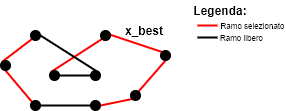
\includegraphics[scale=0.38]{Images/x_best} 
  \caption{\footnotesize{Selezione rami}}
  \label{selezione_rami} 
\end{center} 
\end{figure}

\begin{algorithm}[H]
\DontPrintSemicolon
\KwIn {$\mathtt{model}$= Modello TSP simmetrico senza vincoli di Subtour Elimination \newline
$\mathtt{deadline}$= time limit complessivo dell'algoritmo\newline
$\mathtt{percentage}$= array con i valori delle percentuali di fissagio degli archi\newline
$\mathtt{num_nodi}$= numero di nodi dell'istanza tsp\newline}
\KwOut {$\mathtt{x}$= soluzione intera senza subtour}
\BlankLine
$\mathtt{n \gets}0$\;
\BlankLine
\While{$expired\_time < deadline$}{
 \BlankLine\BlankLine
 $\mathtt{setTimeLimit()}$\;
 $\mathtt{x \gets solve(}model\mathtt{)}$\;
 \BlankLine\BlankLine
 \For{$\mathtt{j \gets}0$ \KwTo $num\_nodi-1$}{
   $k \gets random(0,1)$\;
   \BlankLine\BlankLine
   \If{$  100*k \leq percentage[n\;mod\;leght(percentage)]  $}{
     \BlankLine
     $Aggiungi \;\;\mathtt{x\_best[j]}\;\;to\;\;S\;where\;S=\{edges\;to\;fix\}$
   }
   \BlankLine
}
\BlankLine
\ForAll{$x_{i,j} \in S$}{
$\mathtt{x_{i,j} \gets}1$\;
\BlankLine
}
\BlankLine
$\mathtt{n \gets}n+1$\;
\BlankLine
}
\caption{Hard Fixing}
\end{algorithm}

\subsection{Soft Fixing}\label{soft fixing}
Il metodo seguente fa utilizzo di vincoli aggiuntivi, detti \textbf{Local Branching} e che ha dato il via alla sviluppo della \textbf{Math-Heuristic}, approccio di programmazione matematica (es. tramite CPLEX) unita all'algoritmica euristica\cite{local_branching}.\\
L'approccio utilizzato è simile a quello dell'Hard Fixing, ma la scelta delle variabili da imporre a 1 non viene fatta in maniera randomica ma viene lasciata a CPLEX.\\
Partendo da una soluzione intera ammissibile del TSP $x^H$, viene aggiunto un vincolo sui lati con valore 1 in $x^H$:\\
$$\underset{e\in E\; : \; {x_e}^{H}=1}\sum{x_e}\;\geq\; 0.9\;n$$
dove la sommatoria indica il numero di variabili che vengono preservate a 1 rispetto alla soluzione $x^H$ e \textbf{n} indica il numero di archi selezionati, pari al numero di nodi + 1.\\
In questo caso, il vincolo permetterà a CPLEX di fissare il 90\% dei rami scelti in $x^H$ e avere il 10\% di libertà. Per questo motivo, CPLEX riduce il numero di archi su cui lavorare, in quanto molti nodi hanno già un numero di archi selezionati pari a 2.\\
Un modo alternativo di scrivere lo stesso vincolo è il seguente:
$$\underset{e\in E\; : \; {x_e}^{H}=1}\sum{x_e}\;\geq\; n-k$$
dove k=2,...,20 e rappresenta i gradi di libertà di CPLEX nel raggiungere la nuova soluzione.\\
Ad ogni iterazione viene aggiunto un nuovo local branching, basato sull'attuale soluzione restituita da CPLEX, e rimosso il vincolo aggiunto nell'iterazione precedente.\\
L'unico aspetto negativo di questo metodo riguarda un mancato miglioramento della soluzione da parte di CPLEX in seguito alla sua esecuzione con l'aggiunta del vincolo. Non scegliendo in maniera randomico i lati da selezionare della soluzione precedente, se non dovesse esserci alcun miglioramento del costo e quindi cambiamento della soluzione, i lati selezionati da CPLEX  con il nuovo \textbf{local branching}, sarebbero gli stessi di prima. Per superare tale problema, k viene inizializzata a 2 e, nel caso in cui non dovesse migliorare la soluzione, viene incrementata.\\
Da dati sperimentali, si è appurato come questo metodo aiuti CPLEX a convergere più velocemente alla soluzione ottima e che valori di k superiori a 20 non aiutino a raggiungere risultati migliori.\\
L'aggiunta di un local-branching permette di analizzare in maniera più semplice e veloce lo spazio delle soluzioni. Normalmente per farlo, vengono enumerati gli elementi di questo spazio, generando un numero molto elevatp di possibli soluzioni, considerando che TSP è un problema NP-hard.\\
Definita una soluzione intera ammissibile $x^H$ e utilizzando la distanza di Hamming, vengono definite soluzioni $k-opt$ rispetto ad $x^H$, quelle che hanno distanza k da $x^H$ (vedi Figura \ref{opt}).\\
\begin{figure}[h] 
\begin{center} 
  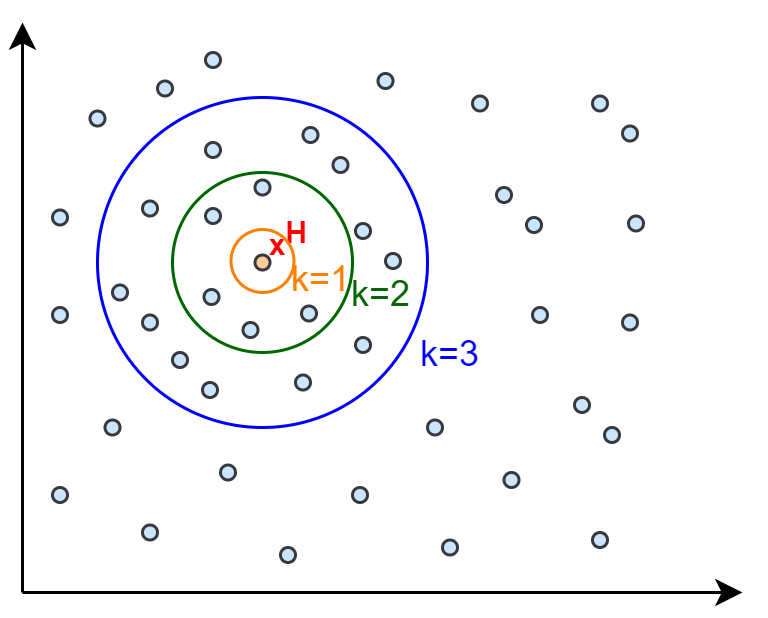
\includegraphics[scale=0.38]{Images/opt}
  \caption{\footnotesize{Spazio delle soluzioni e distanza di Hamming.}} \label{opt} 
\end{center} 
\end{figure}
Se, invece del local branching, venisse utilizzata l'enumerazione delle soluzioni, si dovrebbero generare per \textbf{k} generico circa $n^k$ soluzioni a distanza k da $x^H$ ed in seguito analizzarle tutte per trovare quella con costo minore e migliore di $x^H$.\\
L'utilizzo del local branching può essere adottato con anche problemi generici e non solo con TSP. Di seguito viene riportato l'aprroccio da adottare per generare tutte le soluzioni a distanza minore o uguale di R dalla soluzione euristica di partenza $x_H$:
\begin{align}
& min \{ c^T x:\;\;Ax=b,\;x\in\{0,1\}^n\} \\ \notag \\
& \underset{j\in E:{x_j}^H=0}\sum{x_j}\;+ \underset{j\in E:{x_j}^H=1}\sum{1-x_j}=\; \leq R
\end{align}
dove \textbf{(3.15)} rappresenta la distanza di Hamming dalla nuova soluzione computata $x$ da $x_H$. L'obiettivo del Soft-fixing è cercare di migliorare il costo della soluzione, guardando quelle più vicine possibili a quella attuale. Nella \textbf{Figura \ref{local_exe}} seguito viene riportato un esmpio di una possibile evoluzione dell'algoritmo nella ricerca dell'ottimo, evindenziandone le soluzioni trovate di volta in volta.
\begin{figure}[h] 
\begin{center} 
  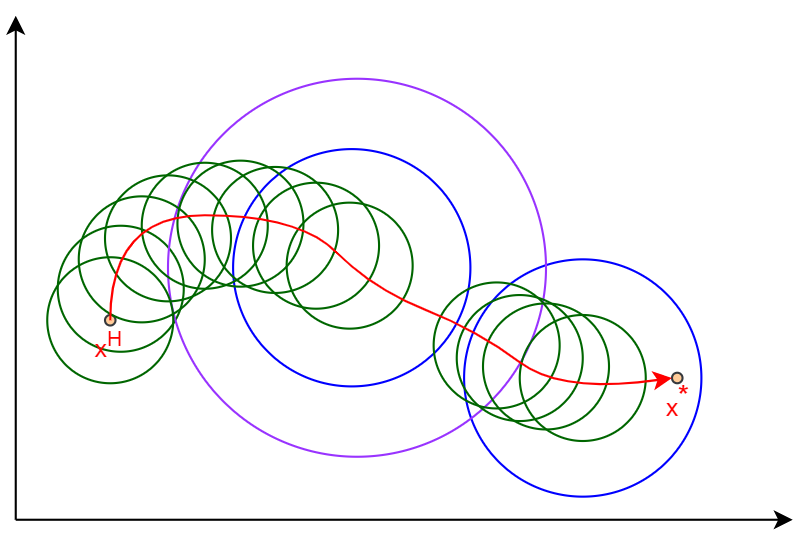
\includegraphics[scale=0.38]{Images/local_exe}
  \caption{\footnotesize{Esempio di esecuzione dell'algoritmo nello spazio delle soluzioni.}} \label{local_exe} 
\end{center} 
\end{figure}
\subsection{Patching algorithm}
Negli algoritmi analizzati nei precedenti capitoli può succedere che CPLEX, prima di restituire la soluzione ottima, computi soluzioni con più componenti connesse. Per evitare che vengano scartate senza essere sfruttate   è possibile utilizzare questo semplice algoritmo euristico che si pone l'obbiettivo di convertirle in una soluzione ammissibile.\\
Date due componenti connesse all'interno della soluzione calcolata, queste vengono unite in una sola grazie all'eliminazione di un ramo ciascuna $\{a, a'\}$ e  $\{b, b'\}$ e alla selezione di altri due rami che fungano da collegamento tra i quattro vertici selezionati ($\{a, b\}$ e $\{a', b'\}$ o $\{a, b'\}$ e $\{a', b\}$) (vedi figura \ref{patching}). 
\begin{figure}[h] 
\begin{center} 
  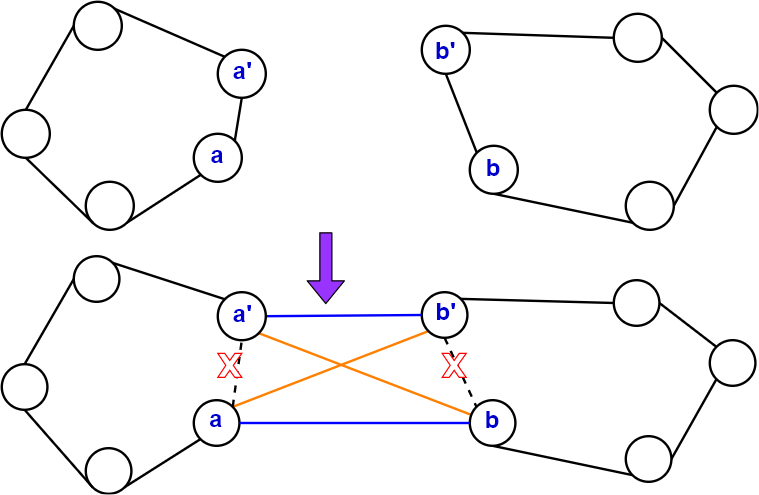
\includegraphics[scale=0.38]{Images/patching}
  \caption{\footnotesize{Esempio di patching}} \label{patching} 
\end{center} 
\end{figure}
Per scegliere quale ramo per ogni componente connessa sia più conveniente eliminare e con quale sia più conveniente sostituirlo, è necessario minimizzare la variazione di costo che quest'operazione comporterebbe, cioè scegliere il minimo tra: \\\\
$min \begin{cases}
\Delta \;(a,b)\;=c_{ab'} + c_{ba'} - c_{aa'} - c_{bb'}\\ 
\Delta' \;(a,b)\;=c_{ab} + c_{b'a'} - c_{aa'} - c_{bb'}\\ 
\end{cases}
\forall \; a,b \in V : comp(a)\neq comp(b)$
\\\\
L'operazione di fusione di due componenti connesse può essere ripetuta finché la soluzione non diventa ammissibile. In questo modo, al termine, è possibile restituire una soluzione accettabile, ma senza garanzia che sia ottima.\\
Nella nostra implementazione è stato scelto di mantenere invariata ad ogni iterazione una delle componenti connesse e di espanderla fondendola a quella più vicina. Grazie a questa scelta viene minimizzato il numero di rami per cui è necessario modificare la struttura dati che li memorizza.\\
Per poter implementare l'algoritmo è necessario utilizzare due diversi tipi di callback messe a disposizione da CPLEX. La prima appartiene alla tipologia delle lazyconstraintcallback  ed è necessaria per ricevere la soluzione trovata dal programma e rielaborarla. A questa soluzione viene applicato l'algoritmo di patching ed il risultato viene memorizzato all'interno in una struttura dati accessibile anche dalla seconda callback dell'utente. Per garantire che la user-callback sia thread-safe, la struttura dati nominata è stata organizzata di  modo tale che ogni thread accedesse ad una sua specifica porzione.\\
La seconda callback necessaria è un heuristic callback e permette all'utente di suggerire a CPLEX una soluzione da cui proseguire la computazione. Questa soluzione sarà quella memorizzata nella struttura dati dalla prima callback e verrà utilizzata dal
programma solo nel caso in cui sia migliore dell'incumbent attuale.\\
Utilizzando, invece, le generic callback non è necessario implementare due diverse user-callback. è sufficiente invocare la callback in due diversi contesti (uno per ricevere la soluzione di cplex, (CPX\_CALLBACKCONTEXT\_CANDIDATE) e l'altro per suggerire il risultato del patching (CPX\_CALLBACKCONTEXT\_LOCAL\_PROGRESS)). I due diversi casi andranno gestiti dall'interno della funzione stessa.\\
Complessivamente il costo di quest'algoritmo è $O(n^2)$, dove $n$ è il numero di nodi.(verificare)

\begin{algorithm}[H]
\DontPrintSemicolon
\KwIn {$\mathtt{x}$= soluzione di un problema di TSP con più componenti connesse\newline}
\KwOut {$\mathtt{y}$= soluzione intera formata da un'unica componente connessa}
\BlankLine
$\mathtt{n\_comps \gets} numero componenti connesse della soluzione$\;
\BlankLine
$\mathtt{c_1\gets}\{0,...,0\}$\;
\BlankLine
\While{$n\_comps > 1$}{
\BlankLine
$\mathtt{c_1 \gets first\_subtour(}x\mathtt{)}$\;
\BlankLine
$\mathtt{c_2 \gets nearest\_subtour(}c_1\mathtt{)}$\;
\BlankLine
$\mathtt{merge\_component(}c_1,c_2\mathtt{)}$\;
\BlankLine
$\mathtt{update(}n\_comps\mathtt{)}$\;
}
$\mathtt{y \gets} c_1$\;
\caption{Patching}
\end{algorithm}